\documentclass[tikz,border=2pt]{standalone}

\usepackage{pgfplots}
\pgfplotsset{compat=1.18}

\begin{document}
	
	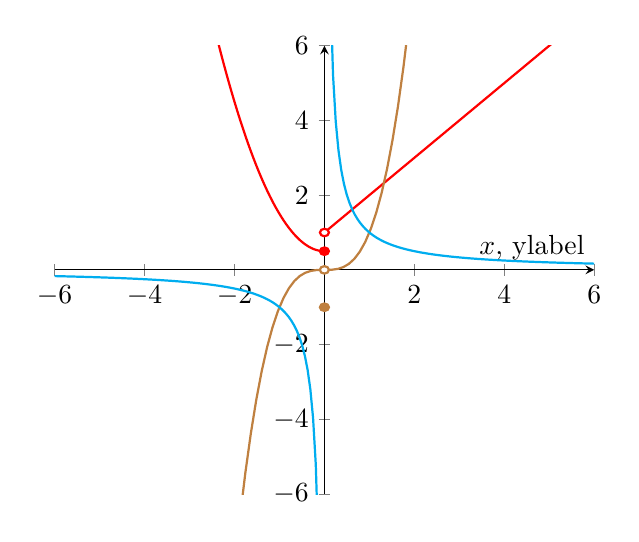
\begin{tikzpicture}
		\begin{axis}[
			xmin=-6,xmax=6,
			ymin=-6,ymax=6,
			axis lines=middle,
			xlabel=$x\text{,}$
			ylabel=$y\text{,}$
			]
			\addplot[thick,domain=0:6, samples=100, color=red]{x+1};
			\addplot[thick,domain=-6:0, samples=100, color=red]{x*x+0.5};
			\addplot[thick,domain=-6:6, samples=100, color=brown]{x*x*x};
			\addplot[thick,domain=0.01:6, samples=100, color=cyan]{1/x};
			\addplot[thick,domain=-6:-0.01, samples=100, color=cyan]{1/x};
			\draw [brown, thick, fill=white] (0,0) circle [radius=0.1];
			\draw [brown, thick, fill=brown] (0,-1) circle [radius=0.1];
			\draw [red, thick, fill=white] (0,1) circle [radius=0.1];
			\draw [red, thick, fill=red] (0,0.5) circle [radius=0.1];
		\end{axis}
	\end{tikzpicture}
	
\end{document}